\chapter{Analisi dei requisiti}
\label{chap:analisi-requisiti}

\section{Casi d'uso}
In avvio di stage sono stati definiti requisiti e interazioni minime tra chi usa il gestionale e il motore di previsione, così da focalizzare solo i casi d’uso necessari alle previsioni.

\subsection{Attori individuati}
Gli attori che interagiscono con il motore di previsione sono:
\begin{itemize}
    \item \textbf{Utente finale}: usa l’interfaccia di ErpAI per avviare previsioni e consultare i risultati.
    \item \textbf{Gestionale ErpAI}: applicazione principale che inoltra le richieste al modulo di previsione via API protette, gestisce autenticazione e memorizza/mostra i risultati.
    \item \textbf{Modulo di previsione}: microservizio che aggiorna i dati, allena il modello, genera previsioni e notifica ErpAI via callback.
    \item \textbf{Modulo chatbot}: microservizio che può interrogare il modulo di previsione via API per ottenere previsioni e spiegazioni da usare nelle risposte.
\end{itemize}
L’interazione è orchestrata da ErpAI, che media verso il modulo di previsione e il chatbot.

\subsection{Casi d'uso}
\begin{center}
    \rowcolors{1}{}{tableGray}
    \begin{longtable}{|p{2.2cm}|p{11.8cm}|}
    \hline
    \multicolumn{1}{|c|}{\textbf{ID}} & \multicolumn{1}{c|}{\textbf{Descrizione}}\\
    \hline 
    \endfirsthead
    \rowcolor{white}
    \multicolumn{2}{c}{{\bfseries \tablename\ \thetable{} -- Continuo della tabella}}\\
    \hline
    \multicolumn{1}{|c|}{\textbf{ID}} & \multicolumn{1}{c|}{\textbf{Descrizione}}\\
    \hline 
    \endhead
    \hline
    \rowcolor{white}
    \multicolumn{2}{|r|}{{Continua nella prossima pagina...}}\\
    \hline
    \endfoot
    \endlastfoot 
    
    UC1 & \textbf{Attori}: Utente finale.\\
        & \textbf{Scopo}: Avviare una richiesta di previsione.\\
        & \textbf{Pre-condizione}: Autenticazione effettuata su ErpAI.\\
        & \textbf{Post-condizione}: Richiesta creata e inoltrata a ErpAI. \\ \hline
    UC1.1 & \textbf{Attori}: Utente finale.\\
        & \textbf{Scopo}: Selezionare l’intervallo temporale per la previsione.\\
        & \textbf{Pre-condizione}: Interfaccia di ErpAI aperta sulla schermata di previsione.\\
        & \textbf{Post-condizione}: Intervallo impostato. \\ \hline
    UC1.2 & \textbf{Attori}: Utente finale.\\
        & \textbf{Scopo}: Confermare e inviare la richiesta.\\
        & \textbf{Pre-condizione}: Parametri configurati (intervallo selezionato).\\
        & \textbf{Post-condizione}: Richiesta inviata a ErpAI. \\ \hline

    UC2 & \textbf{Attori}: Gestionale ErpAI.\\
        & \textbf{Scopo}: Inoltrare la richiesta al modulo di previsione.\\
        & \textbf{Pre-condizione}: Richiesta ricevuta dal frontend, API del modulo raggiungibile.\\
        & \textbf{Post-condizione}: Richiesta inoltrata. \\ \hline
    UC2.1 & \textbf{Attori}: Gestionale ErpAI.\\
        & \textbf{Scopo}: Richiedere token al modulo di previsione.\\
        & \textbf{Pre-condizione}: Credenziali client configurate.\\
        & \textbf{Post-condizione}: Token ricevuto oppure errore di autenticazione. \\ \hline
    UC2.2 & \textbf{Attori}: Gestionale ErpAI.\\
        & \textbf{Scopo}: Inviare la richiesta con token al modulo di previsione.\\
        & \textbf{Pre-condizione}: Token valido, parametri di previsione disponibili.\\
        & \textbf{Post-condizione}: Richiesta accettata o errore ricevuto. \\ \hline

    UC3 & \textbf{Attori}: Modulo di previsione.\\
        & \textbf{Scopo}: Processare la previsione e notificare ErpAI.\\
        & \textbf{Pre-condizione}: Richiesta UC2.2 ricevuta e valida.\\
        & \textbf{Post-condizione}: Previsione elaborata o errore rilevato. \\ \hline
    UC3.1 & \textbf{Attori}: Modulo di previsione.\\
        & \textbf{Scopo}: Elaborare dati e generare previsione.\\
        & \textbf{Pre-condizione}: Richiesta valida.\\
        & \textbf{Post-condizione}: Previsione pronta oppure errore registrato. \\ \hline
    UC3.2 & \textbf{Attori}: Modulo di previsione.\\
        & \textbf{Scopo}: Notificare il completamento a ErpAI.\\
        & \textbf{Pre-condizione}: Processo terminato (successo o fallimento).\\
        & \textbf{Post-condizione}: Stato aggiornato in ErpAI. \\ \hline
    UC3.E & \textbf{Attori}: Modulo di previsione.\\
        & \textbf{Scopo}: Notificare errore a ErpAI.\\
        & \textbf{Pre-condizione}: Errore registrato durante UC3.1.\\
        & \textbf{Post-condizione}: Stato marcato come fallito in ErpAI. \\ \hline

    UC4 & \textbf{Attori}: Modulo Chatbot.\\
        & \textbf{Scopo}: Richiedere contesto previsione.\\
        & \textbf{Pre-condizione}: Chatbot autorizzato verso le API del modulo di previsione.\\
        & \textbf{Post-condizione}: Richieste pronte o dati ricevuti/errore gestito. \\ \hline
    UC4.1 & \textbf{Attori}: Modulo Chatbot.\\
        & \textbf{Scopo}: Preparare richiesta e token.\\
        & \textbf{Pre-condizione}: Credenziali client configurate.\\
        & \textbf{Post-condizione}: Token ricevuto oppure errore di autenticazione. \\ \hline
    UC4.2 & \textbf{Attori}: Modulo Chatbot.\\
        & \textbf{Scopo}: Recuperare dati previsionali via API.\\
        & \textbf{Pre-condizione}: Token valido, ID previsione noto.\\
        & \textbf{Post-condizione}: Dati ricevuti oppure errore gestito. \\ \hline
    UC4.E & \textbf{Attori}: Modulo Chatbot.\\
        & \textbf{Scopo}: Gestire errore API.\\
        & \textbf{Pre-condizione}: Errore nelle chiamate di UC4.1 o UC4.2.\\
        & \textbf{Post-condizione}: Errore registrato, risposta di errore al chiamante. \\ \hline
    \end{longtable}
\end{center}

\begin{figure}[H]
    \centering
    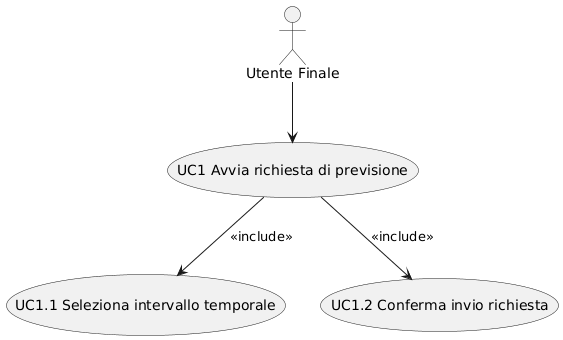
\includegraphics[width=\linewidth]{img/usecase/usecase1.png}
    \caption{Use case 1: avvio e invio richiesta di previsione}
\end{figure}

\begin{figure}[H]
    \centering
    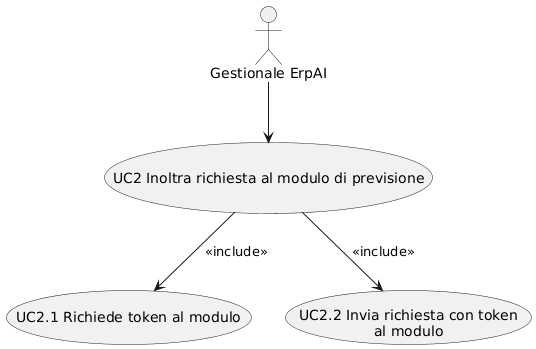
\includegraphics[width=\linewidth]{img/usecase/usecase2.png}
    \caption{Use case 2: inoltro della richiesta da ErpAI al modulo di previsione}
\end{figure}

\begin{figure}[H]
    \centering
    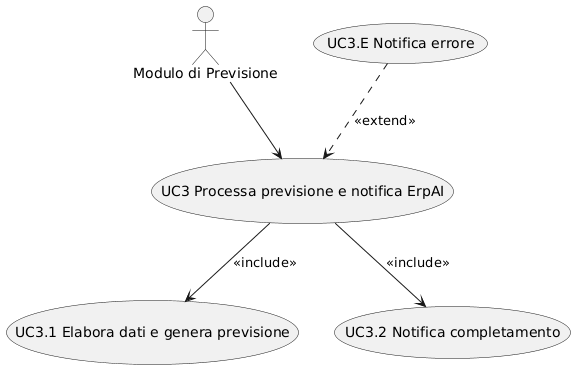
\includegraphics[width=\linewidth]{img/usecase/usecase3.png}
    \caption{Use case 3: elaborazione e notifica da parte del modulo di previsione}
\end{figure}

\begin{figure}[H]
    \centering
    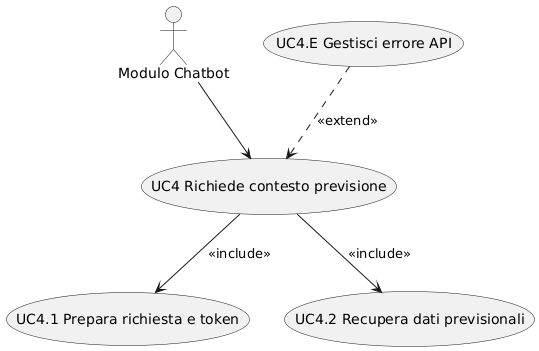
\includegraphics[width=\linewidth]{img/usecase/usecase4.png}
    \caption{Use case 4: interazione del modulo chatbot con il modulo di previsione}
\end{figure}

\section{Requisiti}
Questa sezione raccoglie i requisiti del progetto di previsione e pianificazione per \textit{ErpAI}, organizzati in obbligatori (O), desiderabili (D) e facoltativi (F). La codifica usa un prefisso che identifica la priorità (O/D/F) seguito da un numero progressivo.

\begin{center}
    \rowcolors{1}{}{tableGray}
    \begin{longtable}{|p{2cm}|p{9cm}|p{3cm}|}
    \hline
    \multicolumn{1}{|c|}{\textbf{ID}} & \multicolumn{1}{c|}{\textbf{Descrizione}} & \multicolumn{1}{c|}{\textbf{Categoria}}\\
    \hline 
    \endfirsthead
    \rowcolor{white}
    \multicolumn{3}{c}{{\bfseries \tablename\ \thetable{} -- Continuo della tabella}}\\
    \hline
    \multicolumn{1}{|c|}{\textbf{ID}} & \multicolumn{1}{c|}{\textbf{Descrizione}} & \multicolumn{1}{c|}{\textbf{Categoria}}\\
    \hline 
    \endhead
    \hline
    \rowcolor{white}
    \multicolumn{3}{|r|}{{Continua nella prossima pagina...}}\\
    \hline
    \endfoot
    \endlastfoot 
    
    O01 & Data-set e data-model consolidati. & Obbligatorio \\ \hline
    O02 & Pipeline di previsione con intervalli di confidenza. & Obbligatorio \\ \hline
    O03 & Motore MRP con piani compatibili con lead-time e scorte minime. & Obbligatorio \\ \hline
    D01 & Logica base di feedback learning da input dell’operatore. & Desiderabile \\ \hline
    D02 & Automazione della valutazione delle spiegazioni. & Desiderabile \\ \hline
    D03 & Simulazione dell’impatto delle azioni correttive nel tempo. & Desiderabile \\ \hline
    F01 & Prototipazione grafica per output prescrittivi. & Facoltativo \\ \hline
    F02 & Estensione a scenari multi-macchina. & Facoltativo \\ \hline
    F03 & Integrazione con notifiche real-time per allarmi e azioni. & Facoltativo \\ \hline
    \end{longtable}
\end{center}

\newpage
